\documentclass[10pt,twocolumn,letterpaper]{article}

\usepackage{cvpr} \usepackage{times} \usepackage{epsfig}
\usepackage{graphicx} \usepackage{amsmath} \usepackage{amssymb}
\usepackage{subfig}

% Include other packages here, before hyperref.

% If you comment hyperref and then uncomment it, you should delete
% egpaper.aux before re-running latex.  (Or just hit 'q' on the first
% latex run, let it finish, and you should be clear).
\usepackage[pagebackref=true,breaklinks=true,letterpaper=true,colorlinks,bookmarks=false]{hyperref}


% \cvprfinalcopy % *** Uncomment this line for the final submission

\def\cvprPaperID{****} % *** Enter the 3DIMPVT Paper ID here
\def\httilde{\mbox{\tt\raisebox{-.5ex}{\symbol{126}}}}

% Pages are numbered in submission mode, and unnumbered in
% camera-ready
\ifcvprfinal\pagestyle{empty}\fi
\begin{document}

%%%%%%%%% TITLE
\title{Texture Mapping 3D Models of Indoor Environments with Noisy
  Camera Poses}

\author{First Author\\
  Institution1\\
  Institution1 address\\
  {\tt\small firstauthor@i1.org}
  % For a paper whose authors are all at the same institution, omit
  % the following lines up until the closing ``}''.  Additional
  % authors and addresses can be added with ``\and'', just like the
  % second author.  To save space, use either the email address or
  % home page, not both
  \and
  Second Author\\
  Institution2\\
  First line of institution2 address\\
  {\small\url{http://www.author.org/~second}} }

\maketitle
% \thispagestyle{empty}

%%%%%%%%% ABSTRACT
\begin{abstract}
  Automated 3D modeling of building interiors is useful in
  applications such as virtual reality and environment
  mapping. Applying textures to these models is an important step in
  generating photorealistic visualizations of data collected by
  modeling systems.  Camera pose recovery in such systems often
  suffers from inaccuracies, resulting in visible discontinuties when
  different images are projected adjacently onto a plane for
  texturing. We propose two approaches for reducing discontinuities in
  texture mapping 3d models made of planar surfaces. The first one is
  tile based and can be used where camera axes are at arbitrary angles
  with respect to the plane normals of the surfaces. The second one
  results in a more seamless texture but is only applicable where
  camera axes for imagery are closely aligned with plane normals. The
  effectiveness of our approaches are demonstrated on two indoor
  datasets.
\end{abstract}

%%%%%%%%% BODY TEXT
\section{Introduction}
\label{sec:introduction}
Three-dimensional modeling of indoor environments has a variety of
applications such as training and simulation for disaster management,
virtual heritage conservation, and mapping of hazardous sites. Manual
construction of these digital models can be time consuming, and as
such, automated 3D site modeling has garnered much interest in recent
years.

The first step in automated 3D modeling is the physical scanning of
the environment's geometry. An indoor modeling system must be able to
recover camera poses within an environment while simulatenously
reconstructing the 3D structure of the environment itself
\cite{chen2010indoor, hz, kua2012loopclosure, liu2010indoor}.This is
known as the simultaneous localization and mapping (SLAM) problem, and
is generally solved by taking readings from laser range scanners,
cameras, and inertial measurement units (IMUs) at multiple locations
within the environment.

Mounting such devices on a human-carried platform provides unique
advantages over vehicular-based systems on wheels in terms of agility and
portability, but can also result in much
larger localization error. As a result, common methods for texture
mapping generally produce poor results.

In this paper, we present a number of approaches to texture mapping 3D models of indoor environments made of planar surfaces in the presence of uncertainty and noise in camera poses. In particular, we consider a human-operated backpack system with a number of laser range scanners as well as 2 cameras facing left and right, each equipped with fisheye lenses reaching an approximately 180$^{\circ}$ field of view. Considering that the human operator walks at about 1 meter/second, and images are captured at 5 Hz, there is a considerable amount of overlap between successive images.

With the laser scanners active, the human operator wearing the
backpack takes great care to walk a path such that every wall in the
desired indoor environment is traversed and scanned lengthwise at
least once.

Using data collected by the onboard sensors and applying multiple localization
and loop-closure algorithms \cite{chen2010indoor, kua2012loopclosure,
  liu2010indoor}, the backpack is then localized over its
data collection period. This requires recovering the 6 degrees of freedom for the backpack as well as all its sensors, including the cameras mounted on it. \footnote{In this paper, we use the terms localization and pose recovery interchangeably, in that they both refer to recovering position and orientation.} Once this is complete, the data from the laser range scanners is used to generate a 3D point cloud of the surrounding environment. 
Approximate normal vectors for each point in the
point cloud are then calculated by gathering neighboring points within
a small radius and processing them through principal component
analysis. These normal vectors allow for the classification and
grouping of adjacent points into structures such as walls, ceilings,
floors, and staircases. A RANSAC algorithm is then employed to fit
polygonal planes to these structured groupings of points, resulting in
a fully planar model \cite{sanchez2012point}. This model, consisting
of multiple 2D polygonal planes in 3D space, along with the set of
images captured by the backpack's cameras and their noisy 3D poses,
can be considered the input to our texture mapping problem.

The remainder of the paper is organized as follows. Section
\ref{sec:simpleTextureMapping} describes the general problem of
texture mapping and examines two variants of a tile-based mapping approach and their
shortcomings.  Section \ref{sec:existingApproaches} demonstrates two
previous attempts at improving texture alignment, and demonstrates their
inadequacies for our datasets.  Section \ref{sec:proposedApproach}
presents our proposed approach to texture mapping, combining an
improved localization refinement process with two image selection
approaches. Section \ref{sec:resultsAndConclusions} contains results
and conclusions.

In all subsequent sections, we discuss the process of texture mapping
a single plane, as the texturing of each of our planes is independent
and can be completed in parallel.

\section{Tile-Based Texture Mapping}
\label{sec:simpleTextureMapping}
\begin{figure}
  \centering
  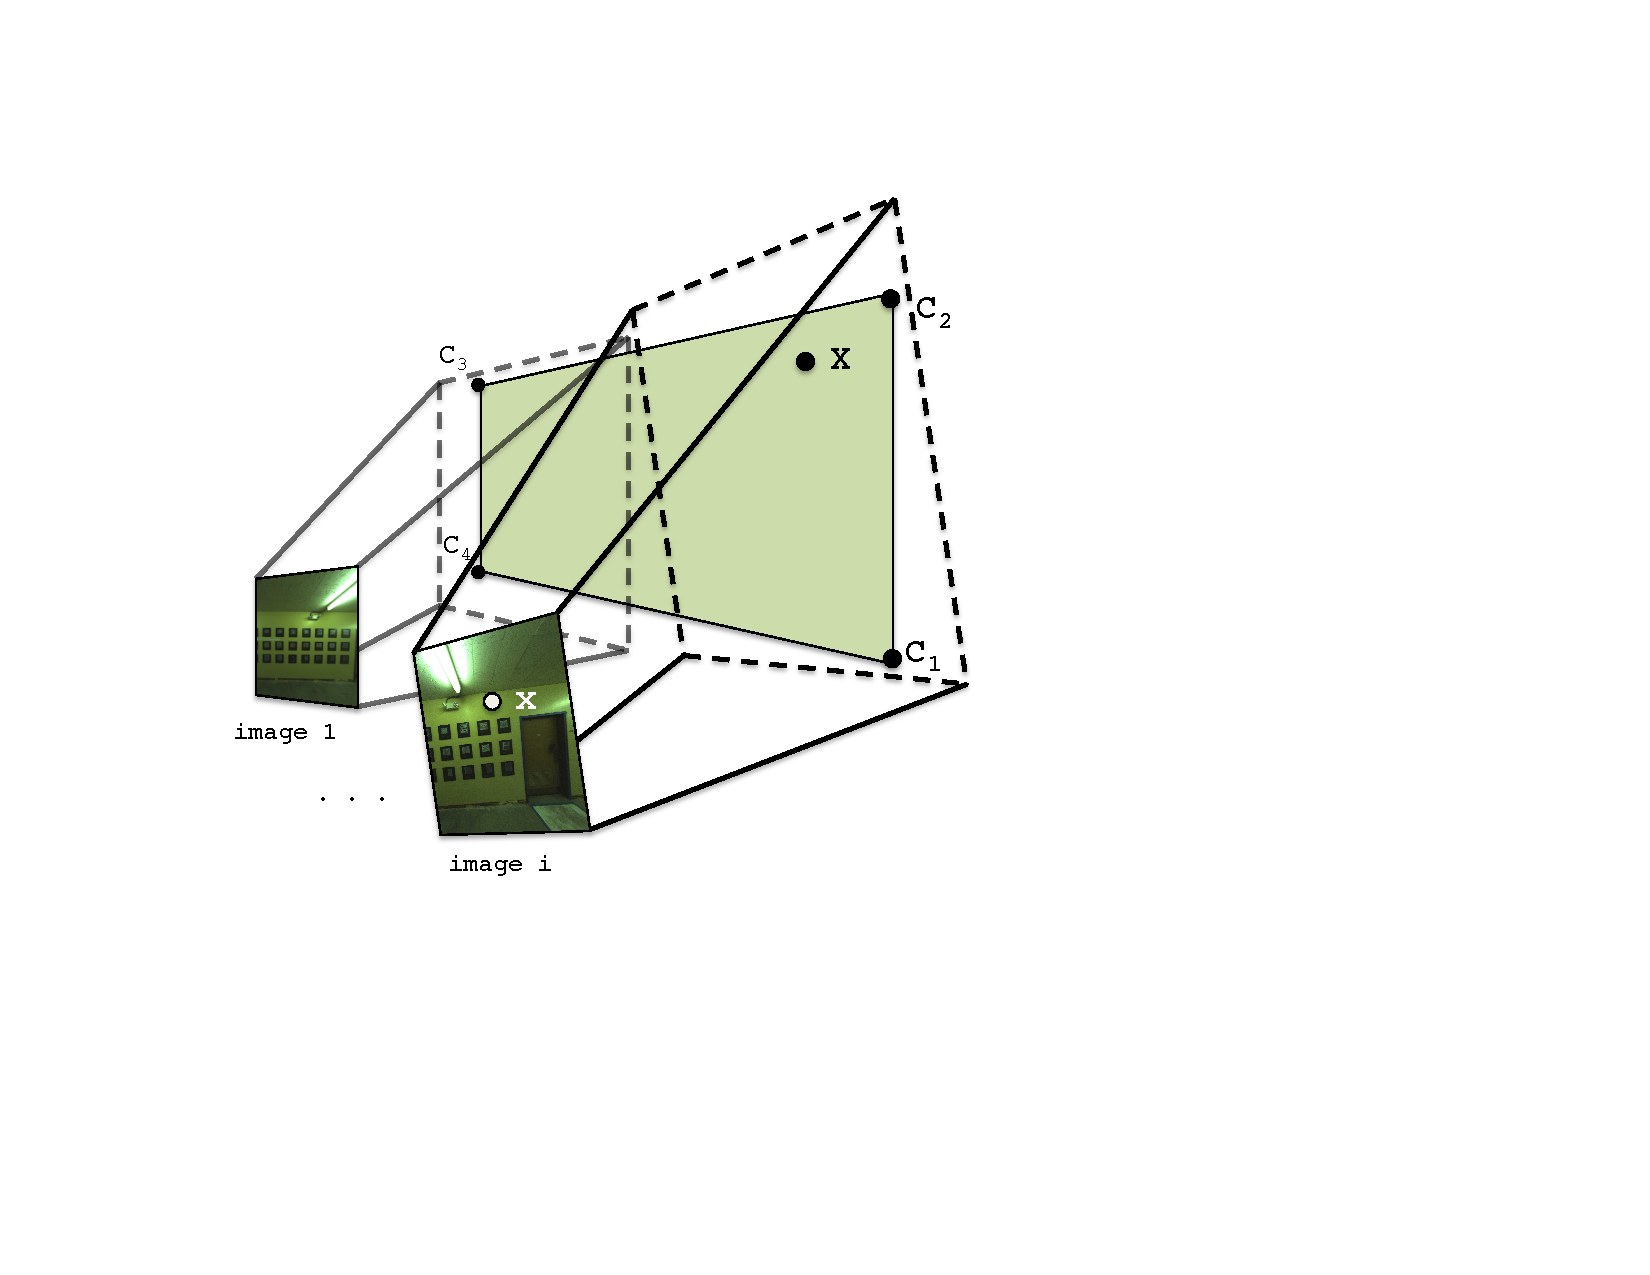
\includegraphics[height=2in]{Projection.pdf}
  \caption{Planes are specified in 3D space by four corners $C_1$ to
    $C_4$. Images are related to each plane through the camera
    matrices $P_{1..M}$. }
  \label{fig:projection}
\end{figure}

The geometry of the texture mapping process for a plane is shown in
Figure \ref{fig:projection}.  As described earlier, we are provided
with a set of $M$ images with which we must texture our target
plane. Each image has a camera matrix $P_i$ for $i=1..M$, which
translates a 3D point in the world coordinate system to a 2D point or
pixel in image $i$'s coordinates. A camera matrix $P_i$ is composed of
the camera's intrinsic parameters, such as focal length and image
center, as well as extrinsic parameters which specify the rotation and
translation of the camera's position in 3D world coordinates at the
time that image $i$ is taken. These extrinsic parameters are
determined by the backpack hardware and localization algorithms
\cite{chen2010indoor, liu2010indoor, kua2012loopclosure} and are quite
noisy.

Our goal is to texture each plane using images captured by the
backpack system, while eliminating any visual discontinuities or seams
that would suggest that the plane's texture is not composed of a
single continuous image.

\subsection{Direct Mapping}
\label{sec:directMapping}

Ignoring the fact that the camera matrices $P_{1..M}$ are inaccurate,
we can texture the plane by discretizing it into small square tiles,
generally about 5 pixels across, and choosing an image to texture each
tile with. We choose to work with rectangular units to ensure that
borders between any two distinct images in our final texture are
either horizontal or vertical. Since most environmental features
inside buildings are horizontal or vertical, any seams in our texture
intersect them minimally and are likely to be less noticeable.

In order to select an image for texturing tile $t$, we must first
gather a list of candidate images that contain all four of its
corners, which we can quickly check by projecting $t$ into each image
using the projection method above. Furthermore, each candidate image
must have been taken at a time when its camera had a clear
line-of-sight to $t$, which can be calculated using standard
ray-polygon intersection tests between the camera location, the center
of $t$, and every other plane, all in world coordinates
\cite{rayintersection}.

Once we have a list of candidate images for $t$, we must define a
scoring function in order to compare images and objectively select the
best one. Since camera localization errors compound over distance, we
wish to minimize the distance between cameras and the plane they
texture. Additionally, we desire images that are projected
perpendicularly onto the plane, maximizing the resolution and amount
of useful texture available in their projections. In other words, we
wish to minimize the angle between the plane normal and the camera
axis for images selected for texture mapping. These two criteria can
be met by maximizing the function $\frac{1}{d} (-1 \cdot \vec{C})
\cdot \vec{N}$ with the parameters shown in Figure
\ref{fig:scoringFunction}. Specifically, $d$ is the distance between
the centers of a camera and a tile, and $\vec{N}$ and $\vec{C}$ are
the directions of the plane's normal and the camera axis respectively.

\begin{figure}
  \centering
  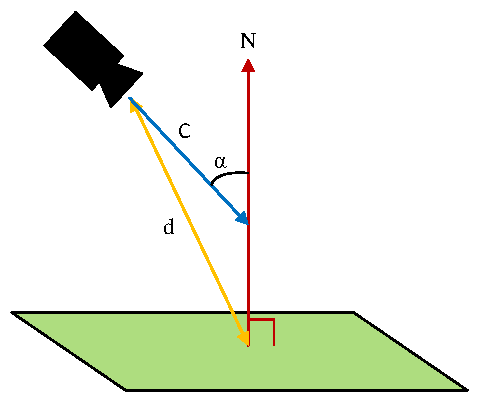
\includegraphics[height=1.5in]{scoringFunction.pdf}
  \caption{We wish to minimize camera angle $\alpha$ and distance $d$}
  \label{fig:scoringFunction}
\end{figure}



\begin{figure}
  \centering
  \subfloat[][]{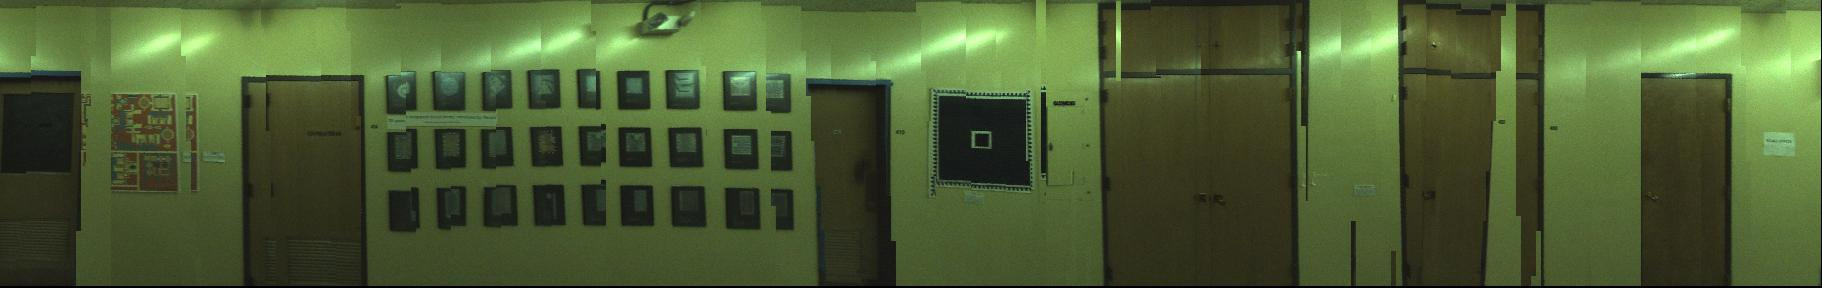
\includegraphics[width=3in]{wall1_naive.jpg}}

  \centering
  \subfloat[][]{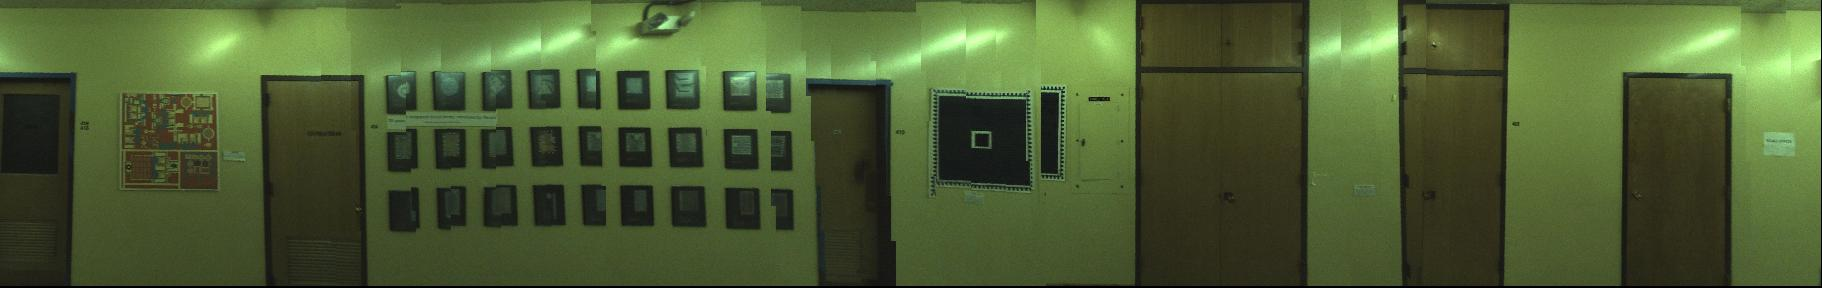
\includegraphics[width=3in]{wall1_cache_full.jpg}}

  \centering
  \subfloat[][]{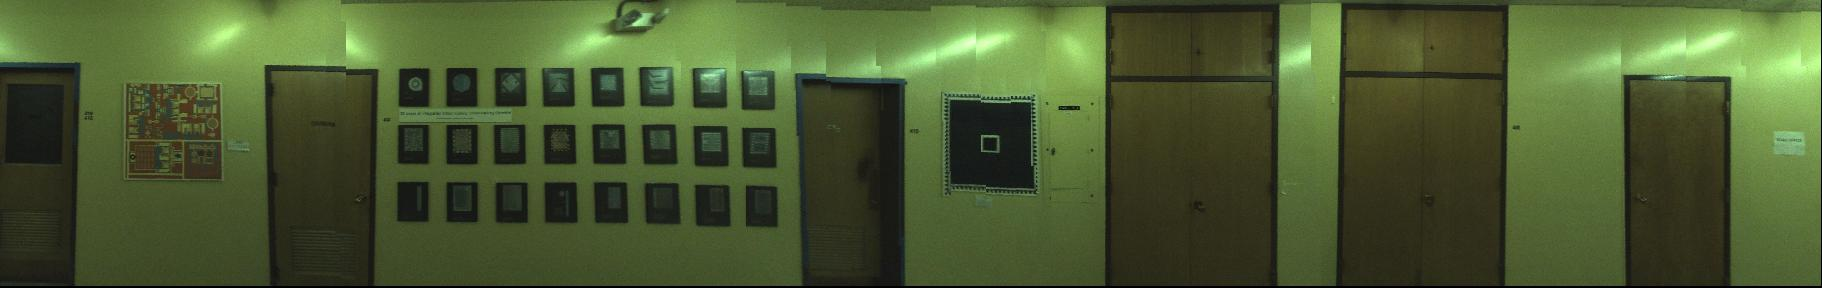
\includegraphics[width=3in]{wall1_cache_full_shifted.jpg}}

  \centering
  \subfloat[][]{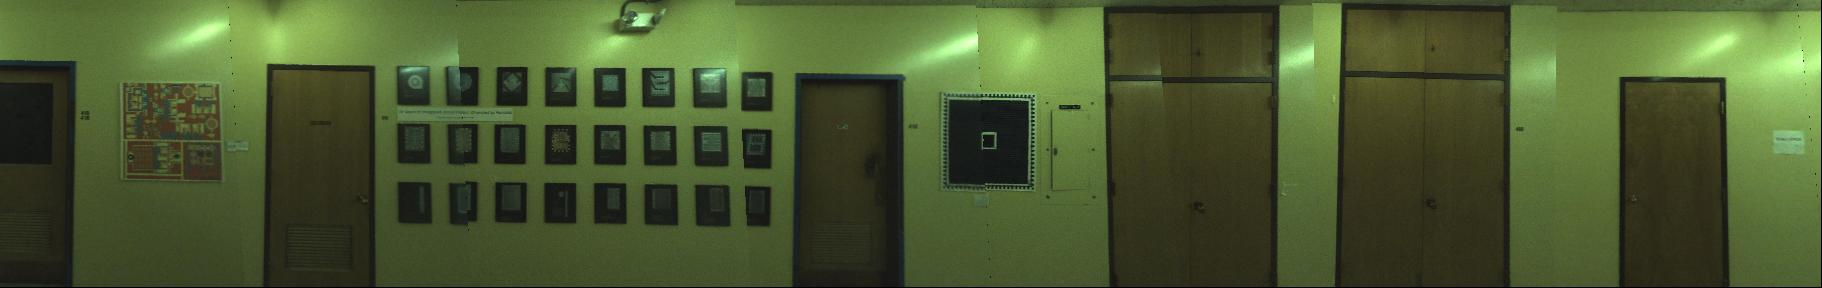
\includegraphics[width=3in]{wall1_dynprog_noblend.jpg}}
  \caption{(a): Direct mapping. (b): Mapping with caching. (c):
    Mapping with caching after image alignment. (d): Seam minimization approach (including image alignment)}
  \label{fig:compareAll}
\end{figure}


As Figure \ref{fig:compareAll}(a) demonstrates, this approach leads
to the best texture for each tile independently, but overall results
in many image boundaries with abrupt discontinuities, due to
significant misalignment between images, as a result of camera pose
inaccuracies.

\subsection{Mapping with Caching}
\label{sec:mappingWithCaching}
Since discontinuities occur where adjacent tiles select non-aligned
images that do not align, it makes sense to take into account image
selections made by neighboring tiles while selecting the best image
for a given tile. By using the same image across tile boundaries, we
can eliminate a discontinuity altogether. If this is not possible
because a tile is not visible in images chosen by its neighbors, using
similar images is likely to result in less noticeable discontinuities.

Similar to a caching mechanism, we select the best image for a tile
$t$ by searching through two subsets of images for a good candidate,
before searching through the entire set. The first subset of images is
those selected by adjacent tiles that have already been textured. We
must first check which images can map to $t$, and then of those, we
make a choice according to the same scoring function. Before reusing
this image, we ensure it meets a threshold, which we set
unconditionally to $\alpha < 45^\circ$, to be considered a viable
image, with $\alpha$ as the camera angle as shown in Figure
\ref{fig:scoringFunction}.

If no satisfactory image is found in the first subset, we then check
our second subset of images, which consists of images that were taken
near the images in the first subset, both spatially and
temporally. These images are not the same as the ones used for
neighboring tiles, but they were taken at a similar location and time,
suggesting that their localization and projection are very
similar. Again, if no good image is found according to the same
threshold, we must then search the entire set of candidate images,
selecting based on the criteria from Figure \ref{fig:scoringFunction}.

The results of this caching approach are shown in Figure
\ref{fig:compareAll}(b). As compared to Figure
\ref{fig:compareAll}(a), discontinuities are reduced overall, but
the amount of remaining seams suggests that image selection alone
cannot produce seamless textures. Camera matrices, or the image
projections themselves have to be adjusted in order to reliably
generate clean textures.

\section{Existing Approaches to Image-Aligned Texture Mapping}
\label{sec:existingApproaches}
In order to produce seamless texture mapping, either camera matrices
need to be refined such that their localization is pixel accurate, or
image stitching techniques need to be applied to provide this
illusion.

Before examining these approaches, we first obtain a set of images to
work with.  Rather than perform camera or image adjustments across the
many thousands of images acquired in a typical data collection, we opt
to work with the more limited set of images corresponding to those
chosen by the direct mapping approach, without caching (Section
\ref{sec:directMapping}. This set of images constitutes a good
candidate set for generating a final seamless texture since it meets
three important criteria. First, each tile on our planeis covered by
at least one image in this set; this ensures no holes in our final
texture. Second, images are all selected according to the scoring
function in Figure \ref{fig:scoringFunction}, ensuring good camera
distances and angles. Third, as a side result of the scoring function,
selected images are only viable candidates for the tiles near their
center of projection. Thus, there should be plenty of overlap between
selected images, allowing for some degree of shifting without
resulting in holes, as well as area for blending between them. With
this set of images, we now review two existing approaches towards
refining and combining their projections.

\subsection{Image Mosaicing}
\label{sec:imageMosaicing}

\begin{figure}
  \centering
  \subfloat[][]{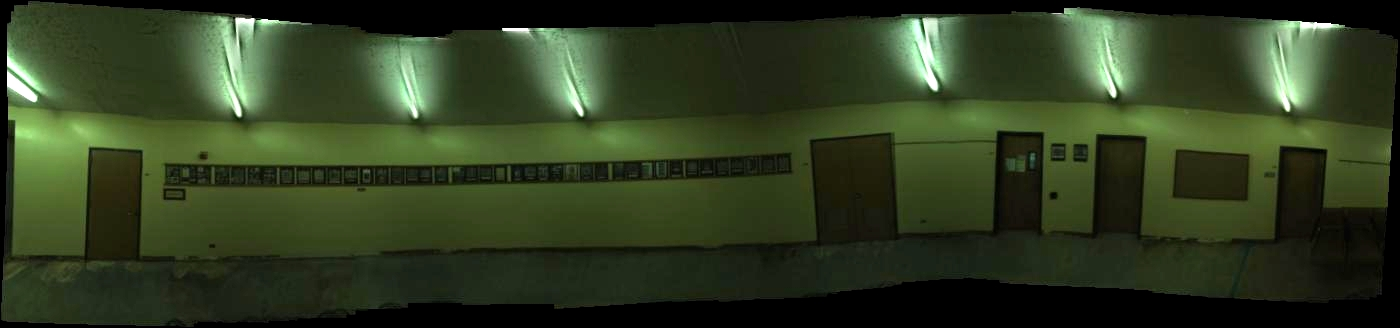
\includegraphics[width=3in]{panoMy.jpg}}

  \centering
  \subfloat[][]{
\includegraphics[width=3in]{Graph_crop.pdf}}
  \caption{Both image mosaicing (a) and the graph-based localization refinement algorithm from
    \cite{chen2010indoor} (b) suffer from the problem of compounding
    errors.}
  \label{fig:mosaic3D}
\end{figure}


When images of a plane are taken from arbitrary overlapping positions,
they are related by homography \cite{hz}. Thus, existing
homography-based image mosaicing algorithms are applicable
\cite{brown2007automatic}. However, errors can compound when long
chains of images are mosaiced together using these approaches. For
example, a pixel in the $n$th image in the chain must be translated
into the first image's coordinates by multiplying by the $3\times3$
matrix $H_1 H_2 H_3 ... H_n$. Any error in one of these homography
matrices is propagated to all further images until the chain is
broken. For some chains of images this can happen almost immediately
due to erroneous correspondence matches and the resulting image mosaic
is grossly misshapen.

Figure \ref{fig:mosaic3D}(a) shows the output of the AutoStitch software
package which does homography-based image mosaicing. This plane is
nearly a best-case scenerio with many features spread uniformly across
it. Even so, the mosaicing produces errors that causes straight lines
to appear as waves on the plane, despite the fact that it was
generated after careful hand tuning. Many planes with fewer features
simply failed outright. Thus, image mosaicing is not a robust enough
solution for reliably texture mapping our dataset.

\subsection{Image-Based 3D Localization Refinement}
\label{sec:imageBased3DRefinement}

Another approach is to refine the camera matrices using image
correspondences to guide the process. Each image's camera matrix has 6
degrees of freedom that can be adjusted. Previous work on this problem
attempted to refine camera matrices by solving a non-linear
optimization problem \cite{liu2010indoor}. This process is specific to
the backpack system which generated our dataset, as it must be run
during backpack localization\cite{liu2010indoor,
  chen2010indoor}. This approach suffers from a similar
error propagation problem as shown in Figure \ref{fig:mosaic3D}(b).


\begin{figure}
  \centering
  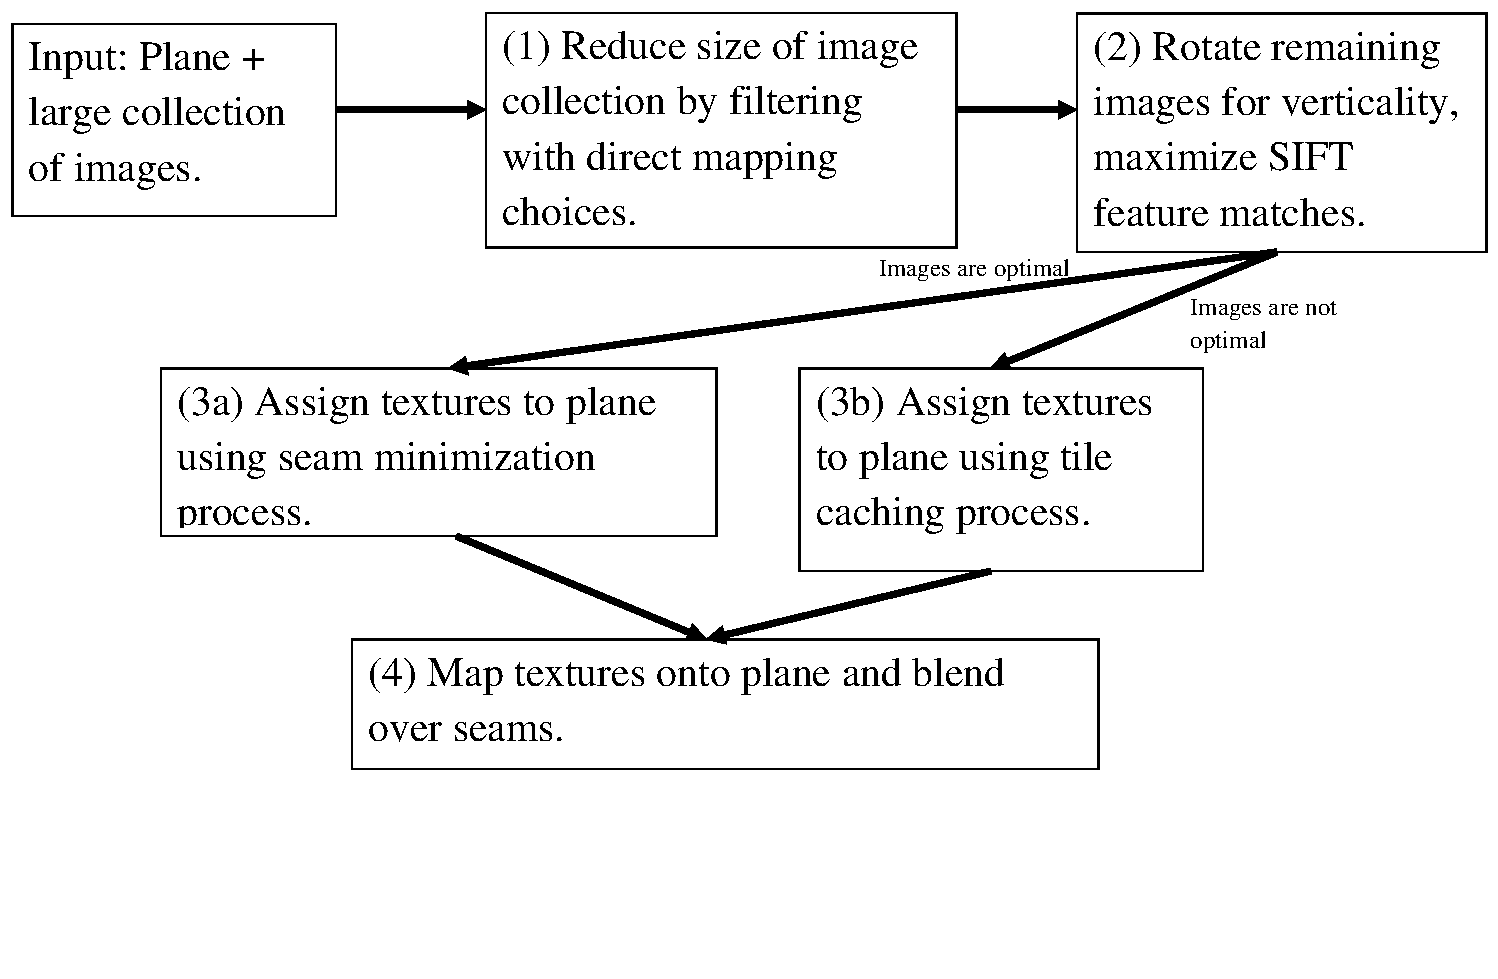
\includegraphics[width=3in]{pipeline.pdf}
  \caption{Our proposed method for seamless texture mapping.}
  \label{fig:pipeline}
\end{figure}


\section{Proposed Method for Seamless Texture Mapping}
\label{sec:proposedApproach}
In this section, we will describe our proposed method for seamless
texture mapping. Our approach consists of 4 steps, as seen in Figure
\ref{fig:pipeline}.  First, we choose a subset of $M$ images to work
with via the direct mapping approach of Section
\ref{sec:directMapping}. Next, we perform image rotation and shifting
in order to maximize SIFT feature matches in overlapping areas between
images. We then project these images onto our plane, applying textures
either with the tile caching method from Section
\ref{sec:mappingWithCaching}, or with the more specialized method to
be described in Section \ref{sec:seamMinimization}. This choice
depends on the availability of head-on images for a given plane. We
then finish by applying linear alphar blending to smooth out any
remaining seams.

\subsection{Image Projection and Rotation}
\label{sec:projectionAndRotation}
We begin with the projection of all images onto the plane. This is
done in the same way as the approaches in Section
\ref{sec:simpleTextureMapping}. We then perform rotations on these
projections, as adjacent images with different orientations result in
strong discontinuities.

These rotations are accomplished by using Hough transforms, which
detect the presence and orientation of linear features in our
images. Rather than match the orientation of such features in each
image, we simply apply rotations such that the strongest near-vertical
features are made completely vertical. This is effective for vertical
planes in indoor models, since they usually consist of parallel
vertical lines corresponding to doors, wall panels, rectangular
frames, etc. If features in the environment are not vertical, or are
not parallel to eachother, this step is skipped.


\subsection{Image Pose Refinement}
\label{sec:robustSIFTFeatureMatching}
Our next step is to align overlapping images by searching for
corresponding points between all pairs of overlapping images using
SIFT feature matching \cite{lowe1999object}. The SIFT matches
determine $dx$ and $dy$ distances between each pair of features for
two images on the plane, though these distances may not always be the
same for different features.

Since indoor environments often contain repetitive features such as
floor tiles or doors, we need to ensure that our SIFT-based distances
are reliable. In order to mitigate the effect of incorrect matches and
outliers, the RANSAC framework \cite{fischler1981random} is used for a
robust estimate of the optimal $dx_{i,j}$ and $dy_{i,j}$ distances between two
images $i$ and $j$. The RANSAC framework handles the consensus-building machinery,
and requires a fitting function and a distance function. For this
application, the fitting function simply finds the average distance
between matches in a pair of images. The distance function for a pair
of points is chosen to be the difference between those points' SIFT match distance
and the average distance computed by the fitting function; we use a 10
pixel outlier threshold. This means that a SIFT match is labeled as an
outlier if its horizontal or vertical distance is not within 10 pixels
of the average distance computed by the fitting function.

We now use the $dx_{i,j}$ and $dy_{i,j}$ distances between each pair of images to refine their positions using least squares. Recall that there are a total of $M^{2}$ possible pairs of images, though we only
generate distances between images that overlap at SIFT feature
points. Given these distances and the original image location
estimates, we can solve a least squares problem
($\textrm{min}_{\vec{\beta}} ||A \vec{\beta} - \vec{\gamma}||_2^2 $)
to estimate the location of the images on the plane. The
$M$-dimensional vector $\vec{\beta}$ represents the unknown $x$ location of each image on the plane for $1 \dots M$. The optimal
$x$ and $y$ locations are obtained in the same way, so we only
consider the $x$ locations here:

\[\vec{\beta} =
\begin{pmatrix}
  x_1, & x_2, & x_3, & \cdots & x_{M-1}, & x_M
\end{pmatrix}
\]

The $N \times (M+1)$ dimensional matrix $A$ is constructed with one row
for each pair of images with measured distances produced by the SIFT
matching stage. A row in the matrix has a $-1$ and $1$ in the columns
corresponding to the two images in the pair. For example, the matrix
below indicates that we generated a SIFT-based distance between images
1 and 2, images 1 and 3, images 2 and 3, etc.

\[
A =
\begin{pmatrix}
  -1 & 1 & 0 & \cdots & 0 & 0\\
  -1 & 0 & 1 & \cdots & 0 & 0\\
  0 & -1 & 1 & \cdots & 0 & 0\\
  \vdots  & \vdots & \vdots & \ddots & \vdots  & \vdots\\
  0 & 0 & 0 & \cdots & 1 & 0 \\
  0 & 0 & 0 & \cdots & -1 & 1 \\
  1 & 0 & 0 & \cdots & 0 & 0 \\
\end{pmatrix}
\]

If only relative distances between images are included then there is
no way to determine the absolute location of any of the images and the
matrix becomes rank deficient. To fix this we choose the first image
to serve as the anchor for the rest, meaning all the absolute
distances are based on its original location. This is done by adding a
row with a $1$ in the first column and the rest zeros.

Finally, the $N$-dimensional observation vector $\vec{\gamma}$ is
constructed using the SIFT-based distances generated earlier in the
RANSAC matching stage. The last element in the observation vector is
the location of the first image determined by its original noisy
localization, from \cite{chen2010indoor, liu2010indoor}. Thus $\vec{\gamma}$ can be written as:

\[
\vec{\gamma}^T =
\begin{pmatrix}
  d_{1,2}, &d_{1,3}, &d_{2,3}, &\hdots &d_{N-2,N-1}, &d_{N-1,N}, &x_1
\end{pmatrix}
\]

The $\vec{\beta}$ that minimizes $||X \vec{\beta} -
\vec{\gamma}||_2^2$ results in a set of image locations on the plane
that best honors all the SIFT-based distance measurements between
images. In practice there are often cases where there is a break in
the chain of images, meaning that no SIFT matches were found between
one segment of the plane and another. In this case we add rows to the
$A$ matrix and observations to the $\vec{\gamma}$ vector that contain
the original noisy $x$ and $y$ distance estimates generated by the
localization algorithm \cite{chen2010indoor, liu2010indoor}. Another
way to do this is to add rows for all neighboring pairs of images and
solve a weighted least squares problem where the SIFT distances are
given a higher weight i.e. 1, and the noisy distances generated by the
localization algorithm \cite{chen2010indoor, liu2010indoor} are given
a smaller weight i.e. 0.01.

After completing this same process for the $y$ dimension as well, and
making the resultant shifts, our images overlap and match each other
with far greater accuracy. Applying the tile caching method from
Section \ref{sec:mappingWithCaching} on these re-localized images
results in the significant improvements shown in Figure
\ref{fig:compareAll}(c), as compared to Figure \ref{fig:compareAll}(b).


\subsection{Seam Minimization}
\label{sec:seamMinimization}

\begin{figure}
  \centering
  \subfloat[][]{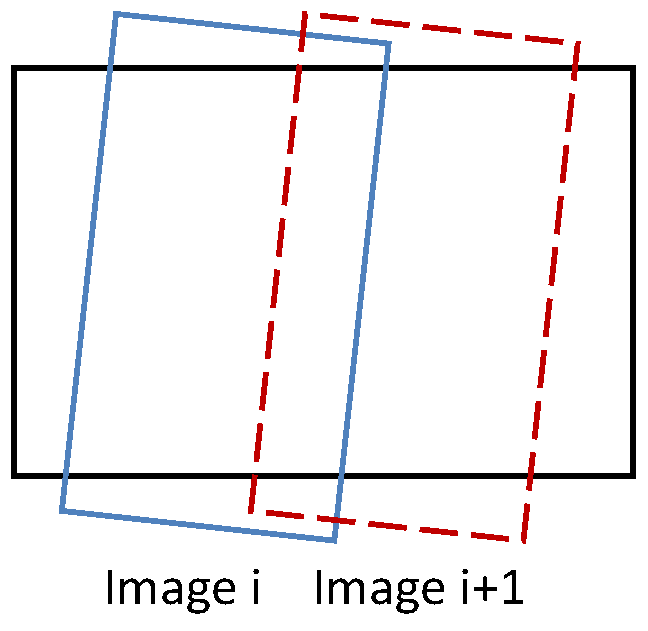
\includegraphics[width=3in]{projectionWall.jpg}}
  \centering
  \subfloat[][]{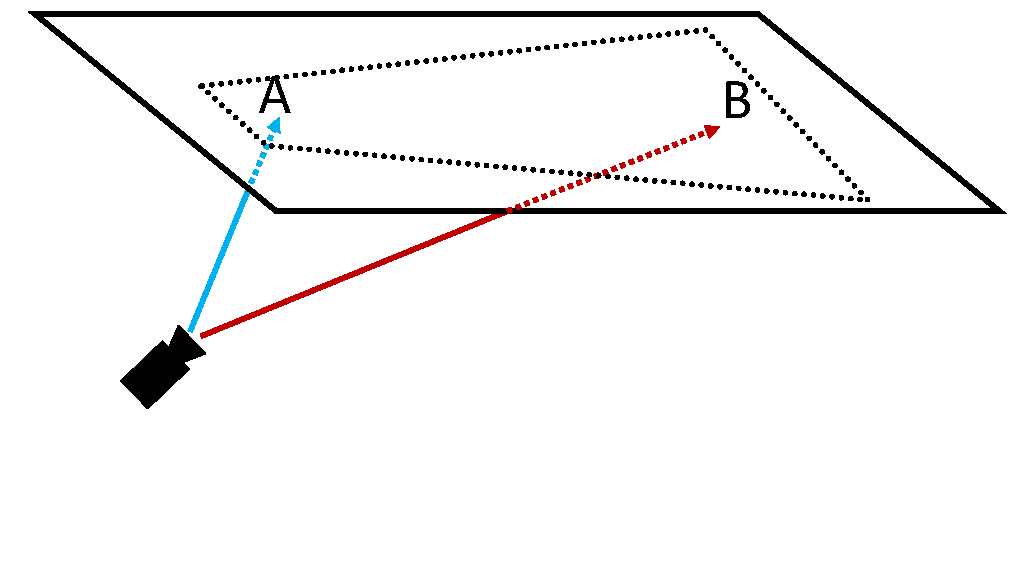
\includegraphics[width=3in]{projectionCeiling.jpg}}
  \caption{(a): Undistorted fisheye images for vertical planes such as
    walls are tilted, but their effective camera axis is more or less
    normal to the plane. (b): The effective camera axis for ceilings
    is at an angle with respect to the plane normal.}
  \label{fig:projectionAngles}
\end{figure}



As mentioned earlier, the mobile backpack system used to capture data
in this paper contains 2 cameras with $180^\circ$ fisheye lenses
facing to the right and left. Since most human operators do not carry
the backpack in a perfectly upright position and are bent forwards at
15 to 20 degrees with respect to the vertical direction, the
undistorted fisheye images are head on with respect to vertical walls,
but at an angle with respect to horizontal floors and ceilings. This
is depicted in Figure \ref{fig:projectionAngles}.


These oblique camera angles translate into textures that span
extremely large areas once projected. Using the tile-based texture
mapping criteria from Figure \ref{fig:scoringFunction}, such
projections have good scores for certain areas on the plane, but worse
scores for others. The tiling approach in Section
\ref{sec:simpleTextureMapping} is thus a good choice for texturing
floors and ceilings, as it uses the parts of image projections that
are good choices for their respective plane locations, e.g. areas near
point A in Figure \ref{fig:projectionAngles}(b), but not near point B.

For wall planes however, most images are taken from close distances
and more or less head-on angles, resulting in higher resolution
fronto-parallel projections. As a result, for each tile on a wall
plane, the cost function of Figure \ref{fig:scoringFunction} is
relatively flat with respect to a large number of captured images, as
they are all more or less head on. Thus it is conceivable to use a
different texturing strategy for walls so as to minimize the visible
seams for texture mapped planes. One way to do so is to choose the
smallest possible set of images that (a) covers the entire plane and
(b) minimizes the amount of visible seams. A straigntforward cost
function that accomplishes the latter is the sum of squared pixel
differences in overlapping regions between all pairs of images, after
they have been aligned as described in Section
\ref{sec:projectionAndRotation}. Minimizing this cost function, which
we refer to as SSD, encourages image boundaries to occur either in
featureless areas, such as bare walls, or in areas where images match
extremely well.

To cover the entirety of a plane, our problem can be defined as
minimally covering a polygon i.e. the plane, using other polygons of
arbitrary geometry i.e. image projections, with the added constraint
of minimizing the cost function between chosen images.  This is a
complex problem, though we can take a number of steps to simplify
it. Given that wall-texture candidate images are taken from more or
less head-on angles, and assuming only minor rotations are made during
localization refinement, we can reason that their projections onto the
plane are approximately rectangular. By cropping them all to be
rectangular, as shown in Figure \ref{fig:projectionAngles}(c), our
problem becomes the conceptually simpler one of filling a polygon with
rectangles, such that the sum of all costs between each pair of
rectangles is minimal. We thus also retain the advantages of working
with rectangular units, as explained in Section
\ref{sec:simpleTextureMapping}.

The location and orientation of the cameras on the acquisition
backpack is such that images nearly always contain the entirety of the
floor to ceiling range of wall planes. Images are therefore rarely
projected with one above another when texturing wall planes. In
essence, we need only to ensure horizontal coverage of wall planes, as
our images provide full vertical coverage themselves. We can thus
construct a Directed Acyclic Graph (DAG) from the images, with edge
costs defined by the SSD cost function, and solve a simple shortest
path problem to find an optimal subset of images with regard to the
cost function \cite{dijkstra}.

\begin{figure}
  \centering
  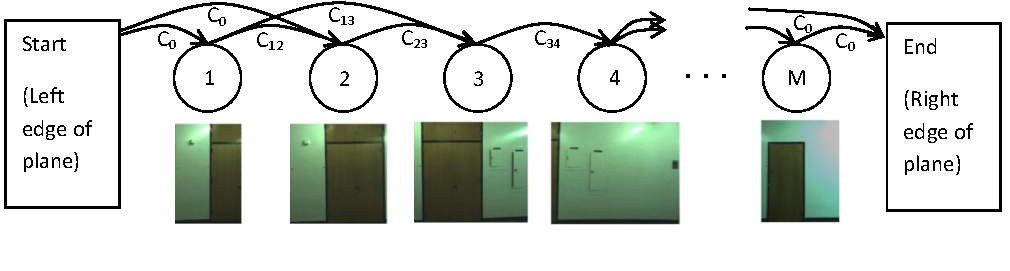
\includegraphics[width=3in]{dagCreation.pdf}
  \caption{DAG construction for the image selection process.}
  \label{fig:dagCreation}
\end{figure}

Figure \ref{fig:dagCreation} demonstrates the construction of a DAG
from overlapping images of a long hallway. Images are sorted by
horizontal location left to right, and become nodes in a
graph. Directed edges are placed in the graph from left to right
between images that overlap. The weights of these edges are determined
by the SSD cost function. Next, we add two
artificial nodes, one start node representing the left border of the
plane, and one end node representing the right border of the
plane. The left(right) artificial node has directed edges with equal
cost $C_0$ to(from) all images that meet the left(right) border of the
plane.

We now solve the shortest path problem from the start node to the end
node. This provides a set of images completely covering the plane
horizontally, while minimizing the cost of seams between images.

In rare cases where the vertical dimension of the plane is not
entirely covered by one or more chosen images, we are left with holes
where no images are selected to texture. To address this, we solve for a new shortest path after modifying the edges chosen by the original shortest path solution such that they
have higher cost than all other edges in our DAG, and solve for a new
shortest path. This ensures that these edges are not chosen again
unless they are the only available option. Our second shortest path
solution results in a new set of chosen images, of which we only
retain those that cover areas not covered by the first set. This
process can be repeated as many times as needed, until holes are no
longer present. This method is not as optimal as a 2D-coverage
solution would be, but it is a fast approximation, and adequately
handles the few holes we encounter.

With this completed, we have now mapped every location on the plane to
at least one image, and have minimized the number of images, as well
as the discontinuities between their borders. Figures \ref{fig:compareAll}(c) and
\ref{fig:compareAll}(d) compare the tile caching method against this
seam minimization method. For the latter, we arbitrarily choose one image for texturing where images overlap. Though both methods provide aligned texturing, the seam minimization approach results in fewer
visible discontinuities, since it directly reduces the cost of each
image boundary, while the tile caching method uses a scoring function
that only approximates this effect. Furthermore, seam minimization
guarantees the best selection of images, while the sequential tile
caching method may select images early on that turn out to be poor
choices once subsequent tiles have been processed. The seam
minimization approach is also less intensive in terms of memory usage
and runtime, as it does not require discretizing planes or images.

In the context of texturing an entire 3D planar model, we apply the seam
minimization approach on walls, due to its superior output when
provided with head-on images. Floors and ceilings however, given their
many images taken at oblique angles, are textured using the tile caching method.

\subsection{Blending}
\label{sec:blending}
We now apply the same blending process to the two texturing methods:
localization refinement followed by either tile caching or seam
minimization.

Although the preprocessing steps and image selection in both methods
attempt to minimize all mismatches between images, there are occasional
unavoidable discontinuities in the final texture due to different
lighting conditions or inaccuracies in planar geometry or
projection. These can however be treated and smoothed over by applying
alpha blending over image seams.  Whether the units we are blending
are rectangularly-cropped images or rectangular tiles, we can apply
the same blending procedure, as long as we have a guaranteed overlap
between units to blend over.

For the tile caching method, we can ensure overlap by texturing a
larger tile than needed for display. For example, for a rendered tile
$l_1 \times l_1$, we can associate it with a texture $(l_1 + l_2)
\times (l_1 + l_2)$ in size. For the seam minimization method, we have
already ensured overlap between images. To enforce consistent blending
however, we add a minimuum required overlap distance while solving the
shortest path problem in Section
\ref{sec:seamMinimization}. Additionally, if images overlap in a region
greater than the overlap distance, we only apply blending over an area
equal to the overlap distance.

After blending pixels linearly across overlapping regions using alpha
blending, texture mapping is complete. Figure
\ref{fig:pipelineimages} shows each incremental step of our texture
mapping approach for a different wall, as well as the final blended output resulting from
both of our methods.

\begin{figure}
  \centering
  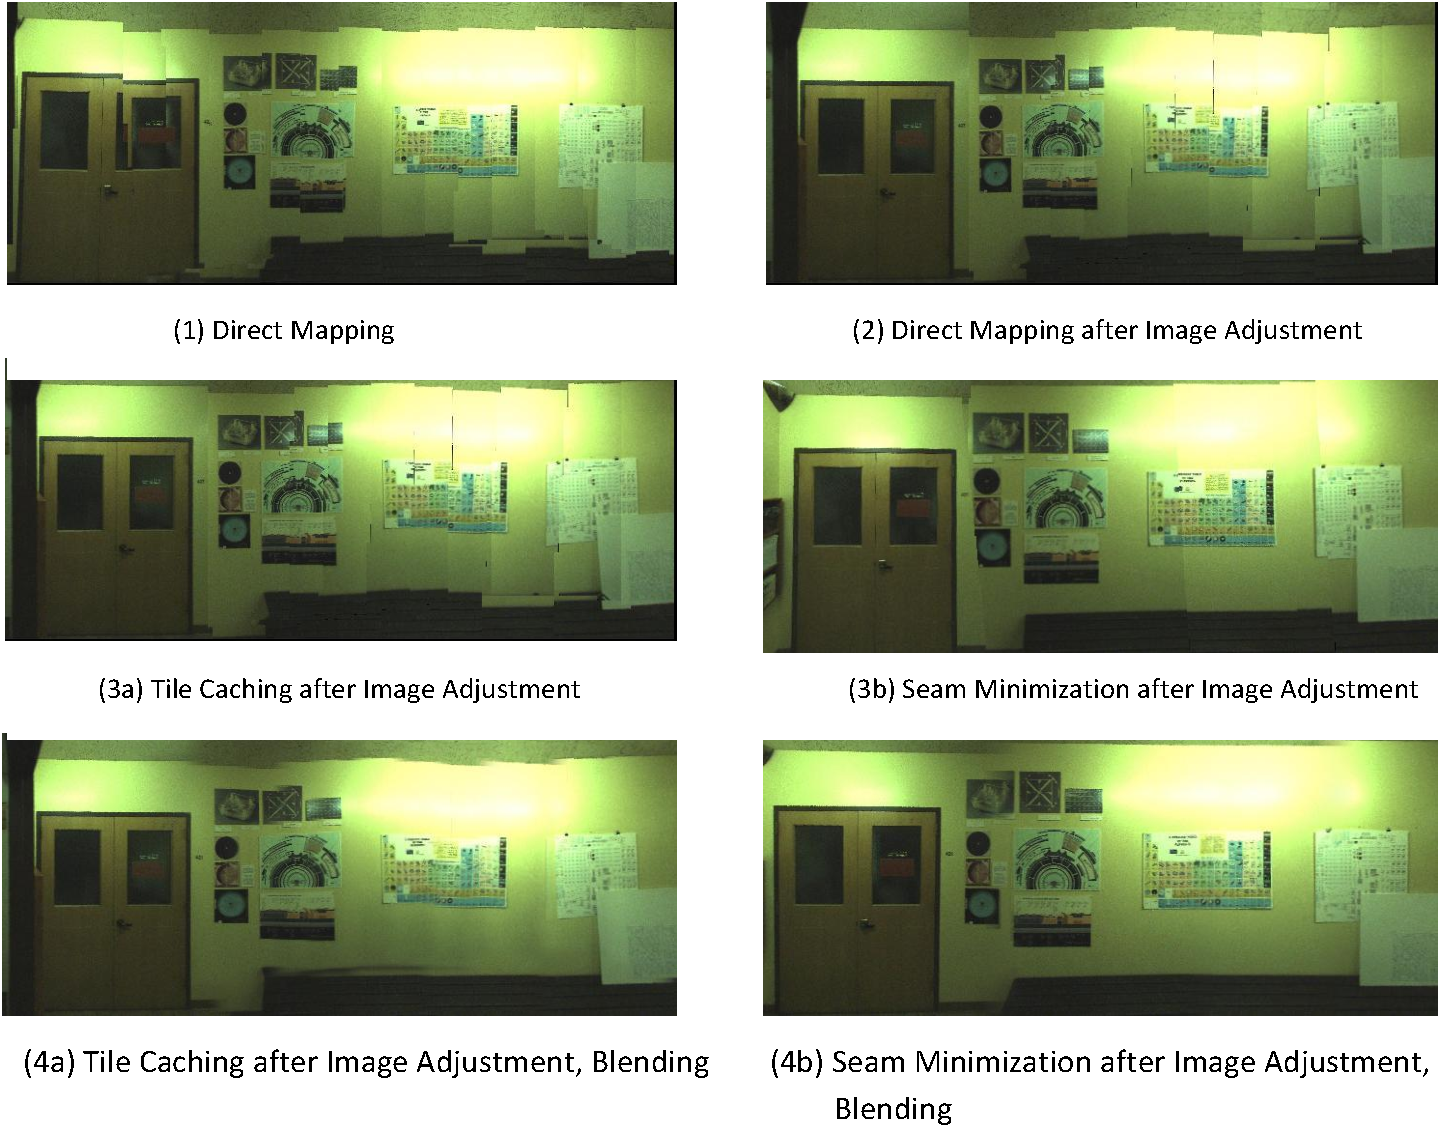
\includegraphics[width=3in]{pipelineimages.pdf}
  \caption{Textures corresponding to each step in our texture mapping
    pipeline.}
  \label{fig:pipelineimages}
\end{figure}


\section{Results and Conclusions}
\label{sec:resultsAndConclusions}
In this paper, we have developed an approach to texture map models
with noisy camera localization data. We are able to refine image
locations based on feature matching, and robustly handle outliers. The tile-based mapping approach can be used to texture both simple rectangular walls as
well as complex floor and ceiling geometry. We also presented a seam minimization texturing method that produces seamless textures on planes where
multiple head-on images are available. Each of these approaches is
highly modular, and easily tunable for different environments and
acquisition hardware.

Examples of ceilings and floors textured with the tile caching approach, and walls
textured with the seam minimization approach, are displayed in Figure
\ref{fig:results}. High resolution texture comparisons, as well as a
walkthrough of a fully textured 3D model are available in the
accompanying video to this paper.

\begin{figure}
  \centering
  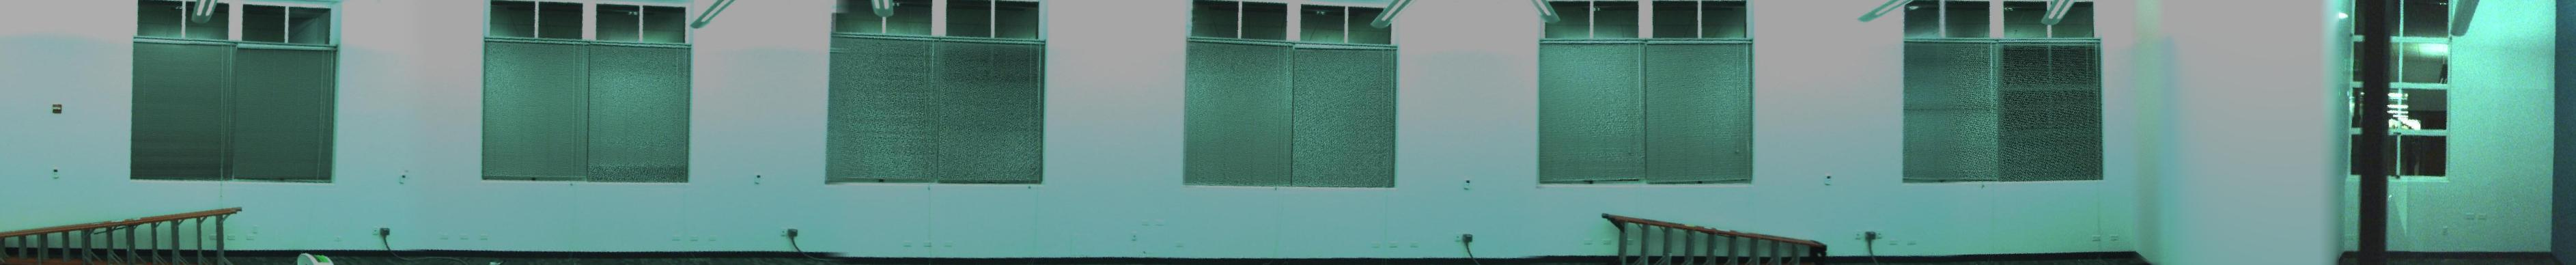
\includegraphics[width=3in]{4thfloor21.jpg}
  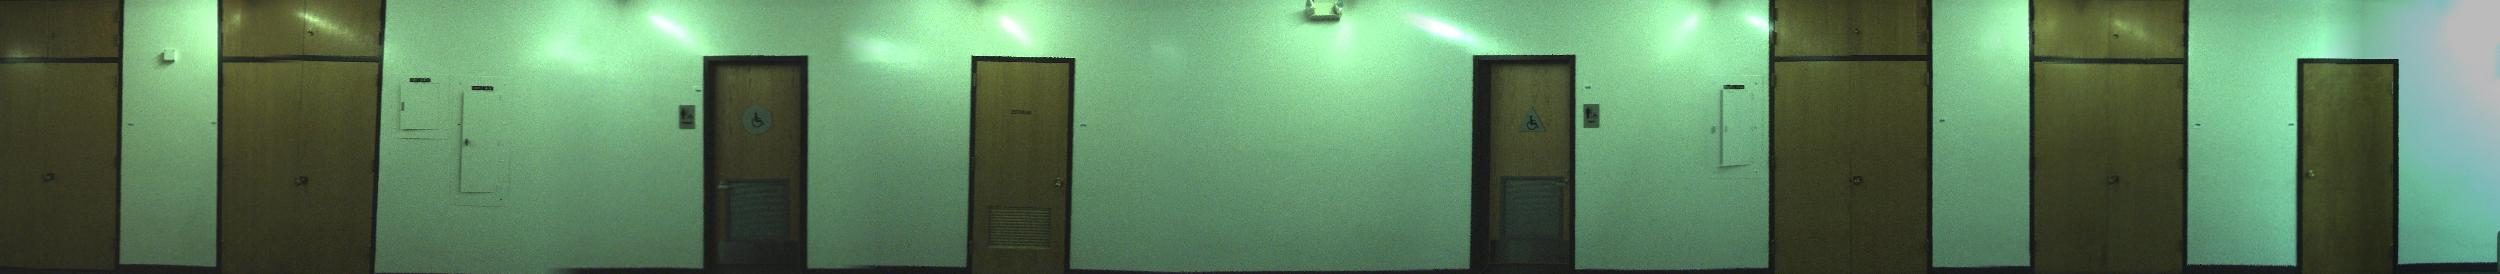
\includegraphics[width=3in]{4thfloor61.jpg}
  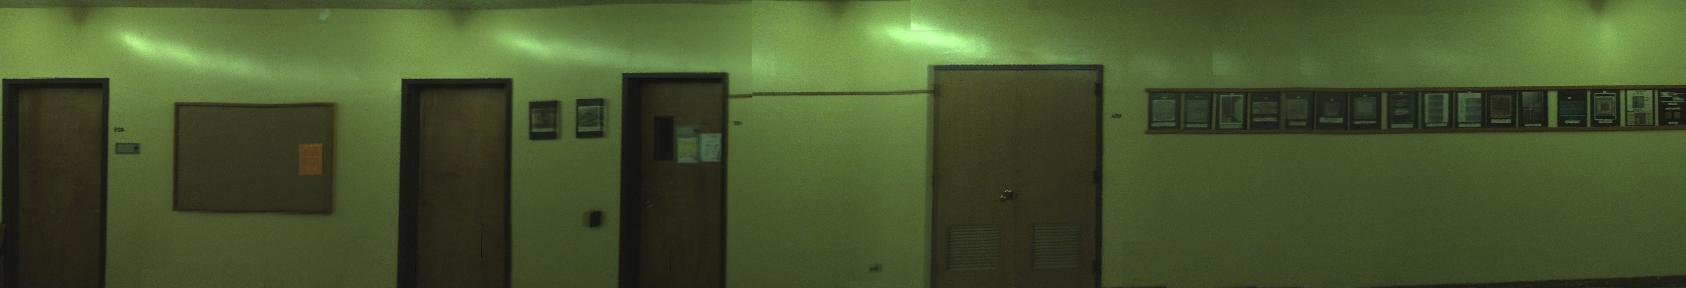
\includegraphics[width=3in]{wall3final.jpg}
  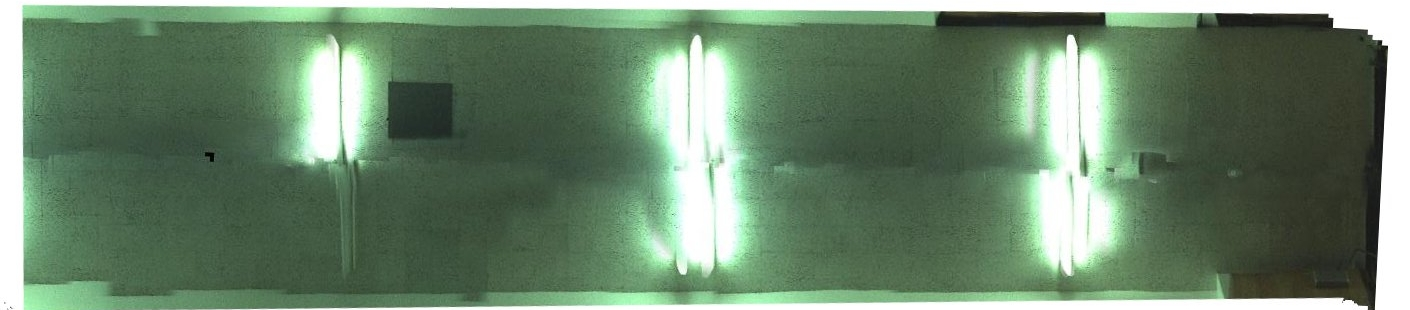
\includegraphics[width=3in]{4thfloor8.jpg}
  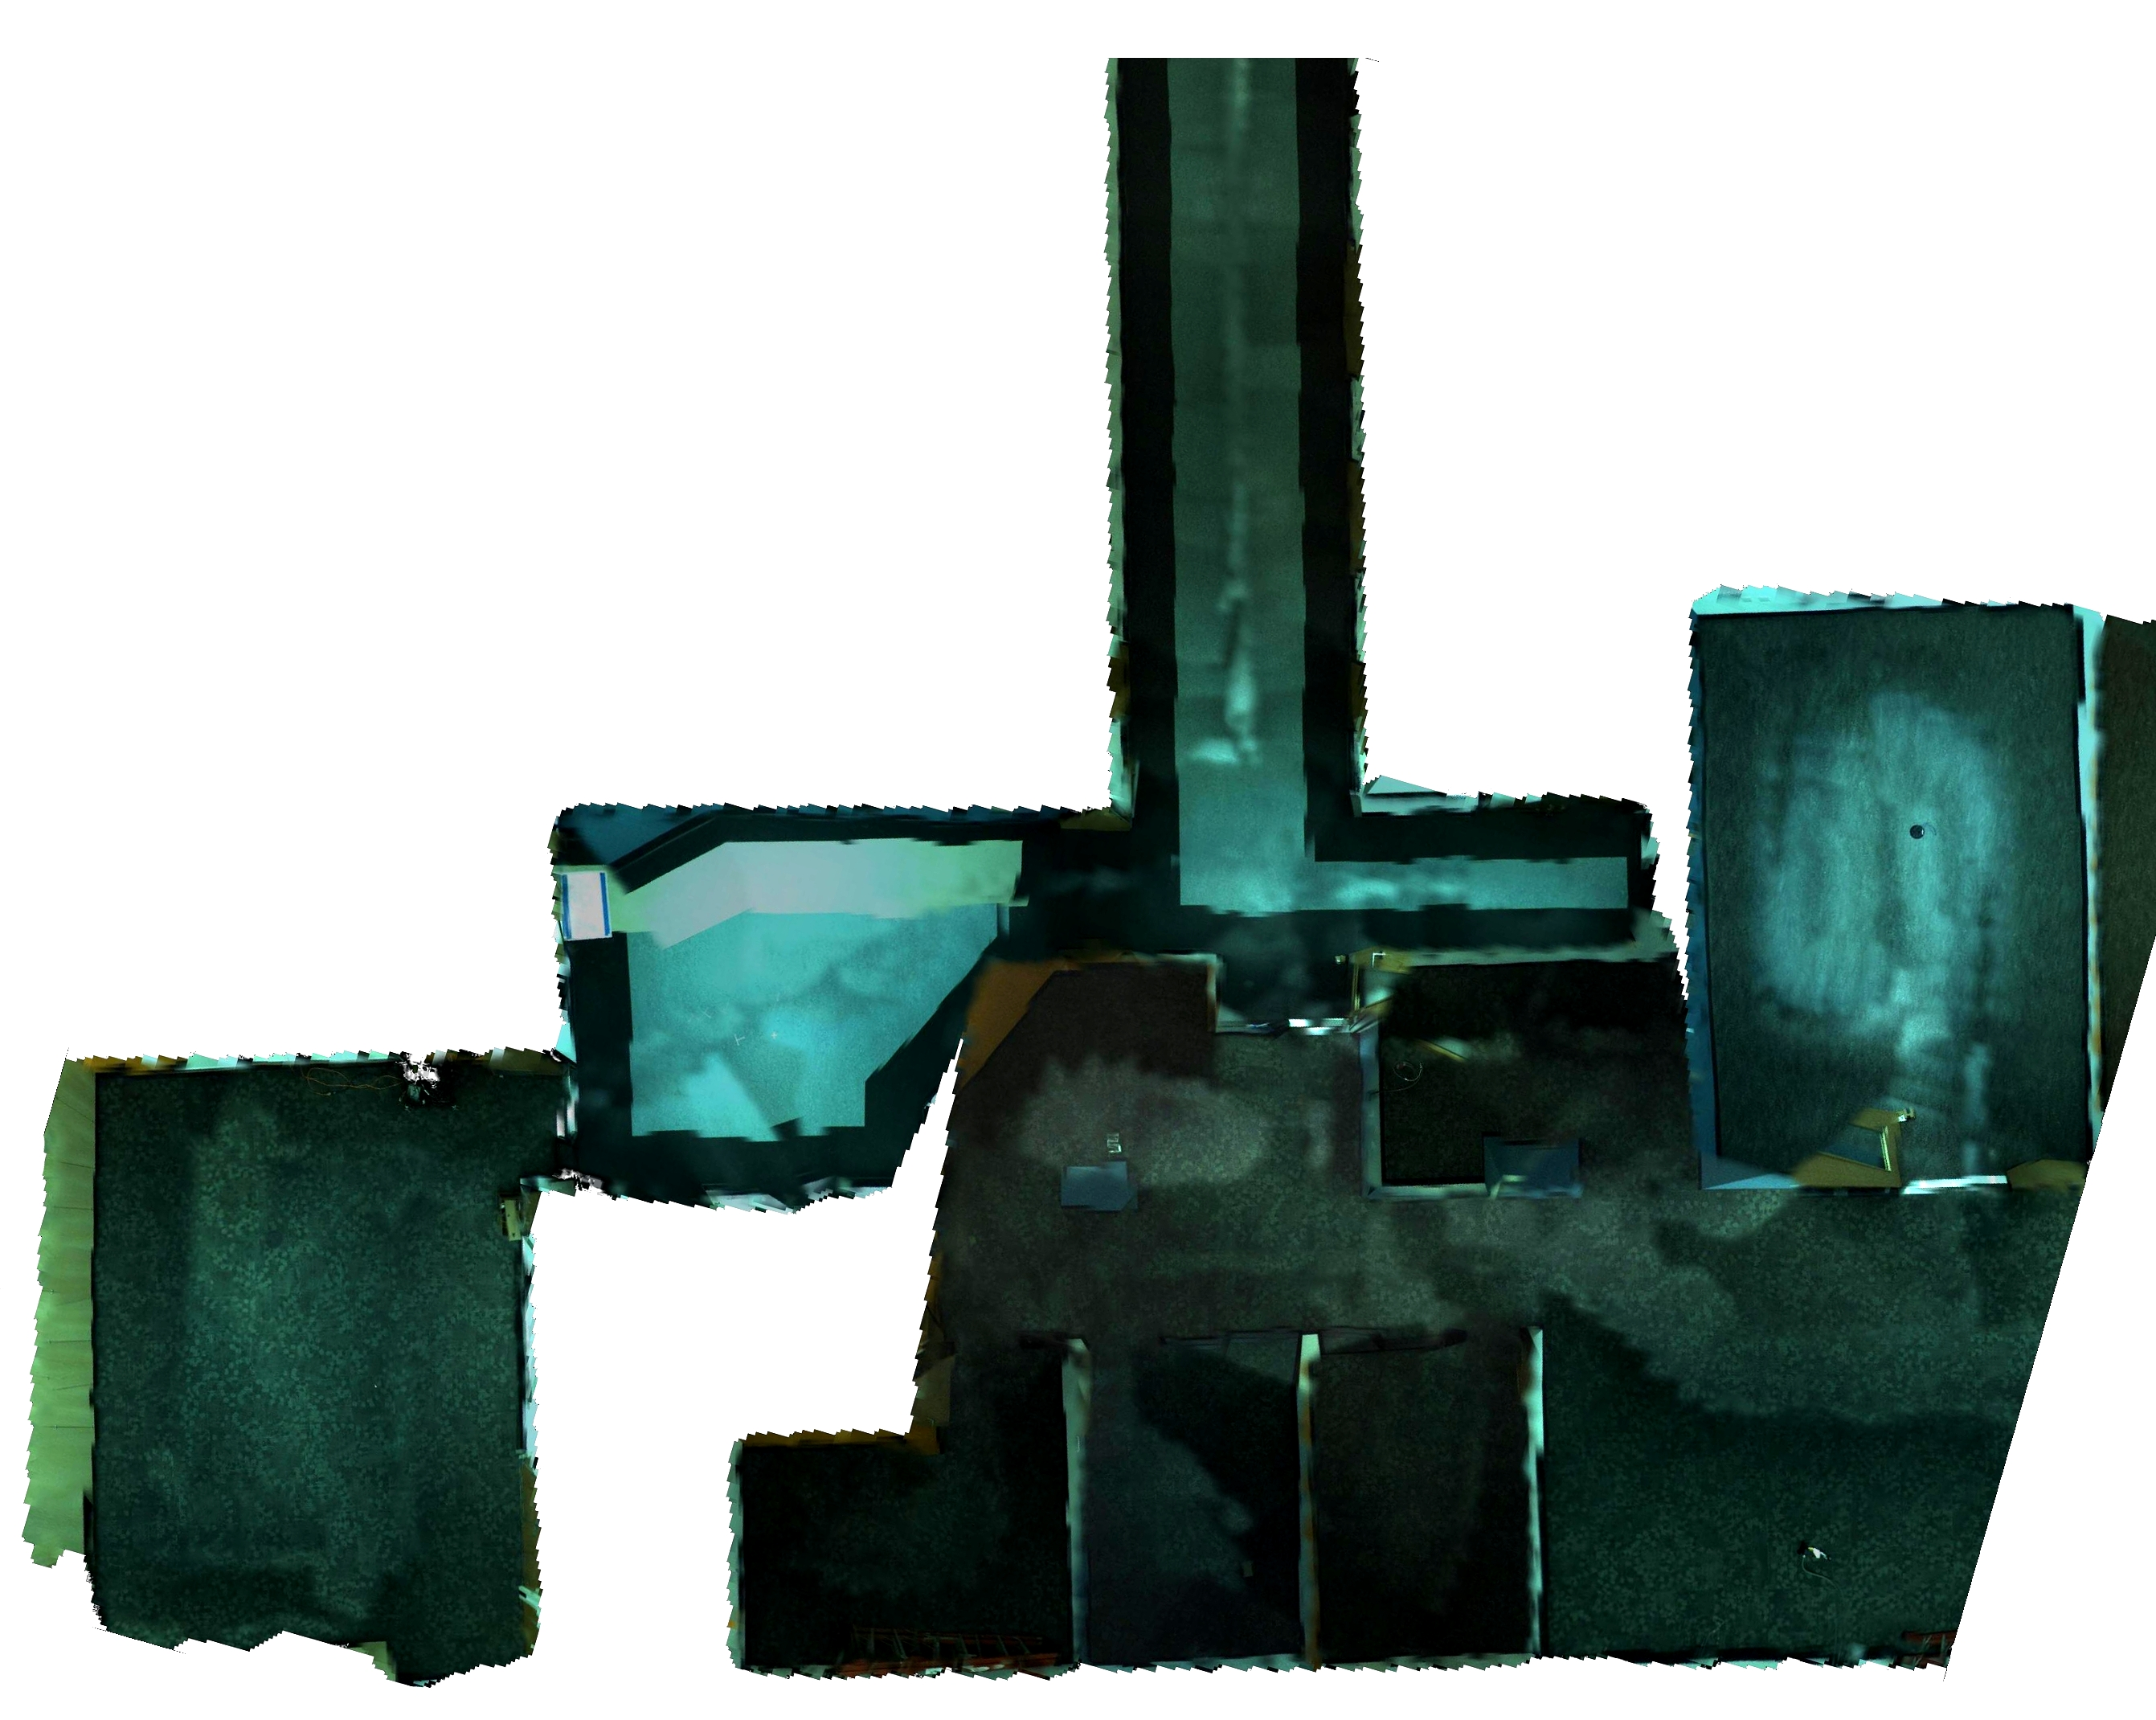
\includegraphics[width=3in]{floorcropped.jpg}
  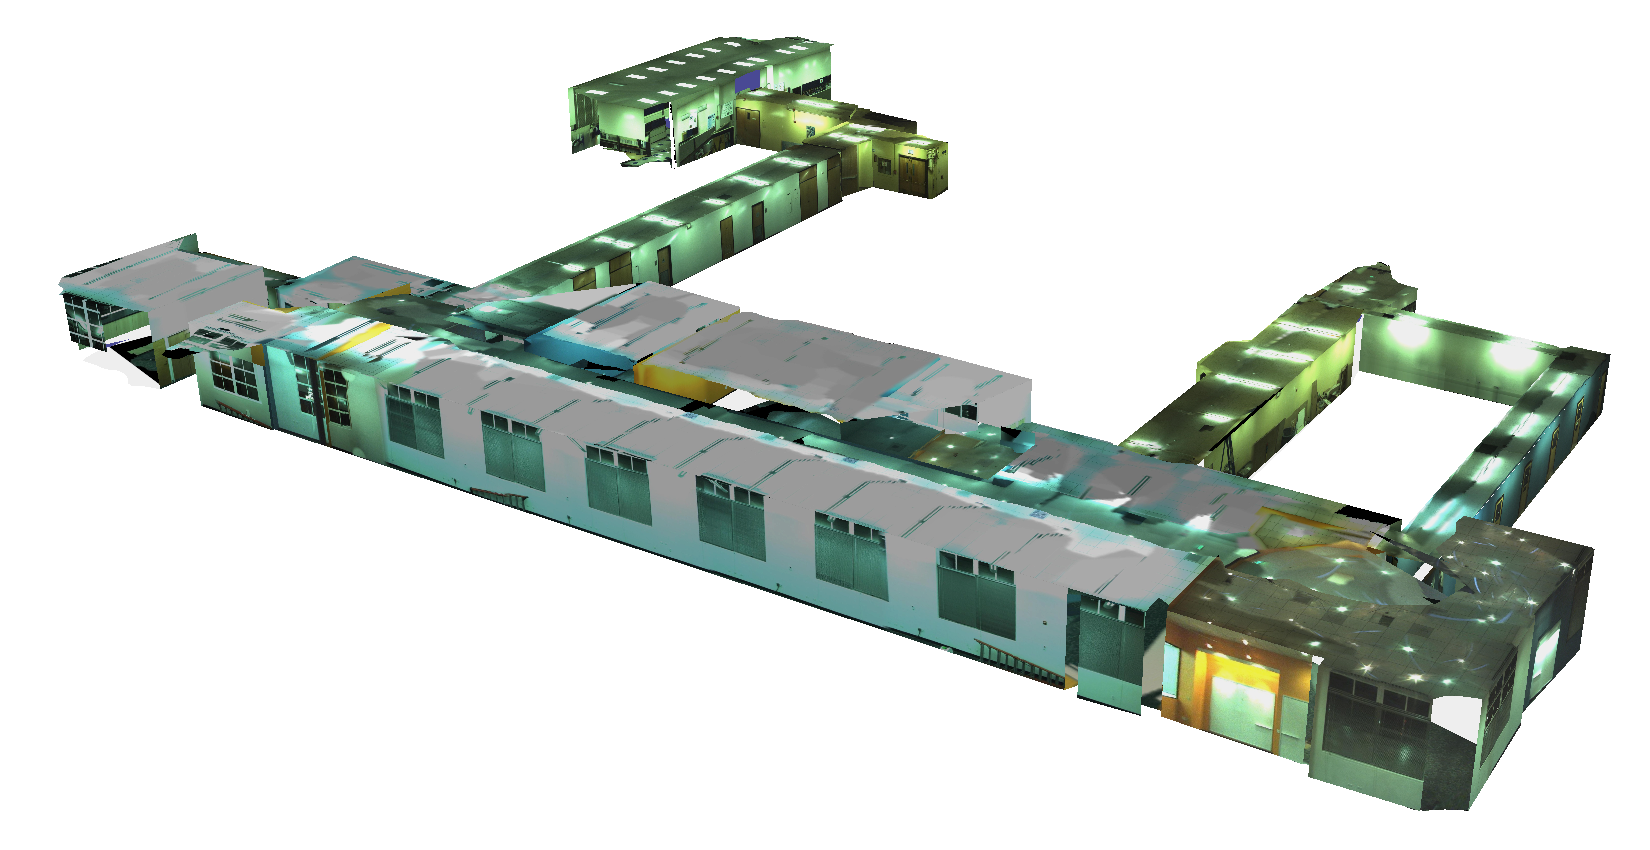
\includegraphics[width=3in]{fullmodel.png}
  \caption{Examples of our final texture mapping output for walls, a
    ceiling, an entire floor, as well as a fully textured model}
  \label{fig:results}
\end{figure}

{\small \bibliographystyle{ieee} \bibliography{egbib} }


\end{document}
